%%%%%%%%%%%%%%%%%%%%%%%%%%%%%%%%%%%%%%%%%
% Journal Article
% LaTeX Template
% Version 1.3 (9/9/13)
%
% This template has been downloaded from:
% http://www.LaTeXTemplates.com
%
% Original author:
% Frits Wenneker (http://www.howtotex.com)
%
% License:
% CC BY-NC-SA 3.0 (http://creativecommons.org/licenses/by-nc-sa/3.0/)
%
%%%%%%%%%%%%%%%%%%%%%%%%%%%%%%%%%%%%%%%%%
%----------------------------------------------------------------------------------------
% PACKAGES AND OTHER DOCUMENT CONFIGURATIONS
%----------------------------------------------------------------------------------------
\documentclass[twoside]{article}
\usepackage{lipsum} % Package to generate dummy text throughout this template
\usepackage[sc]{mathpazo} % Use the Palatino font
\usepackage[T1]{fontenc} % Use 8-bit encoding that has 256 glyphs
\linespread{1.05} % Line spacing - Palatino needs more space between lines
%\usepackage{microtype} % Slightly tweak font spacing for aesthetics
\usepackage[hmarginratio=1:1,top=32mm,columnsep=20pt]{geometry} % Document margins
\usepackage{multicol} % Used for the two-column layout of the document
\usepackage[hang, small,labelfont=bf,up,textfont=it,up]{caption} % Custom captions under/above floats in tables or figures
\usepackage{booktabs} % Horizontal rules in tables
\usepackage{float} % Required for tables and figures in the multi-column environment - they need to be placed in specific locations with the [H] (e.g. \begin{table}[H])
\usepackage{hyperref} % For hyperlinks in the PDF
\usepackage{lettrine} % The lettrine is the first enlarged letter at the beginning of the text
\usepackage{graphicx} % Used for including images
\graphicspath{ {./images/} }
\usepackage{capt-of}
\usepackage{subcaption}
\usepackage{abstract} % Allows abstract customization
\usepackage{array}
\renewcommand{\abstractnamefont}{\normalfont\bfseries} % Set the "Abstract" text to bold
\renewcommand{\abstracttextfont}{\normalfont\small\itshape} % Set the abstract itself to small italic text
\usepackage{titlesec} % Allows customization of titles
\renewcommand\thesection{\Roman{section}} % Roman numerals for the sections
\renewcommand\thesubsection{\Roman{subsection}} % Roman numerals for subsections
\renewcommand\thesubsubsection{\Roman{subsubsection}}
\titleformat{\section}[block]{\large\scshape\centering}{\thesection.}{1em}{} % Change the look of the section titles
\titleformat{\subsection}[block]{\large}{\thesubsection.}{1em}{} % Change the look of the section titles
\usepackage{fancyhdr} % Headers and footers
\pagestyle{fancy} % All pages have headers and footers
\fancyhead{} % Blank out the default header
\fancyfoot{} % Blank out the default footer
\fancyhead[C]{CSCI 4830/7000 $\bullet$ Fall 2019 $\bullet$ Thanika Reddy}  % Custom header text
\fancyfoot[RO,LE]{\thepage} % Custom footer text
% Lorem Ipsum text ala https://hipsum.co/
%----------------------------------------------------------------------------------------
% TITLE SECTION
%----------------------------------------------------------------------------------------
\title{\vspace{-15mm}\fontsize{24pt}{10pt}\selectfont\textbf{An Analysis of the Popularity of Facebook News Posts}} % Article title
\author{
\large
\textsc{Thanika Reddy} \\% Your name
\normalsize University of Colorado Boulder \\ % Your institution
\normalsize \href{mailto:thanika.reddy@colorado.edu}{thanika.reddy@colorado.edu} % Your email address
\vspace{-5mm}
}
\date{}
%----------------------------------------------------------------------------------------
\begin{document}
\maketitle % Insert title
\thispagestyle{fancy} % All pages have headers and footers
%----------------------------------------------------------------------------------------
% ABSTRACT
%----------------------------------------------------------------------------------------
\begin{abstract}
\noindent This study uses the Facebook News Dataset to assess the effect of various factors on the popularity of news posts on Facebook. The insights gained can aid in the creation of posts that reach a wider audience and can also lead to a better understanding of what social media users look for in a post. Predictive analysis was performed using multivariate linear regression, MARS and SVR using an RBF kernel. MARS  improves  the  R\textsuperscript{2} score  by  12.7\% over Multivariate Linear Regression, and SVR further improves it by 14.2\%. Multivariate Linear Regression chooses the number of reactions received by a post to be the most predictive feature, while MARS takes the sentiment of the post into account and chooses the number of "sad" reactions received by a post per second to be the most predictive feature. 
\end{abstract}
%----------------------------------------------------------------------------------------
% ARTICLE CONTENTS
%----------------------------------------------------------------------------------------
\begin{multicols}{2} % Two-column layout throughout the main article text
\section{Introduction}
Content on social media is shared in many different forms, such as status updates, tweets, images, posts and pages. Some shared content becomes more popular and reaches a larger audience than some other content. The popularity of this content can be measured by the number of likes, shares and comments it receives. There can also be different factors that influence the popularity of content, such as the number of followers or friends the creator of the content has, how active those followers are, the number of followers a page the content is posted to has, the day a post is created on, the time it is created at and its sentiment. 

The popularity of content posted on social media has been widely studied. In [1], hierarchical regression is used to study the categories of antecedents that can be related to a Facebook post's popularity. The popularity of news posts on Twitter is analyzed and an exponential regression model is used to predict this popularity in [2]. The sentiment of posted content has also been found to affect its popularity and reach. The rate of information diffusion is higher for content with negative sentiment [3]. Sentiment features extracted from images posted on social media are used to predict the popularity of the image in [4].

This paper studies the factors that determine the popularity of news posts on Facebook. The distributions of various predictor variables are first studied. Following this, the relationships between the predictor variables and outcome are studied. Then, three predictive models (multivariate linear regression, MARS and SVR) are fit to the data. Their performance and the importance they assign to features are used to further analyze what factors determine the popularity of posts and in what manner. 

By indicating what posts should contain and where they should be posted in order to gain more popularity, this study can aid in the creation of posts that reach a wider audience. By indicating what a user looks for in a post before they share or "like" it, these insights can also aid in studies of the psychology of social media users.
%------------------------------------------------
\section{Data}
The Facebook News Dataset [5] is employed in this study. It contains 19,850 Facebook posts from 83 different news organizations and personalities representing up to the last 250 page posts made as of July 14th, 2017. Each post has up to 100 comments for a total of 1,025,403 comments. 

Each post is represented by the following features in the dataset: post creation time, post scrape time, description, link, contents of the post, page ID (of the page the post is on), post ID, number of "angry", "haha", "like", "love", "sad" and "wow" reactions the post had at the time it was scraped and the number of shares the post had. 

Additional features of interest were derived from these features. The post creation time was used to determine the day of the week each post was created, which was one-hot encoded to create seven features. The post creation time was also used to determine the segment of the day each post was created. This created four additional one-hot encoded features that indicate if a post was created between 1 AM and 7 AM, 7 AM and 10 AM, 10 AM and 5 AM or 5 AM and 1 AM. 

The duration for which a post existed before being scraped was calculated using the difference between the post creation time and post scrape time. This was then used to calculate the average number of shares and average number of reactions (of each type) the post received per second, which resulted in a total of seven additional features. The fraction of reactions that were a certain type ("angry", "haha", "like", "love", "sad" or "wow") on each post were also calculated and this resulted in six additional features. 

The Python VADER library was used to perform sentiment analysis on each post, and this resulted in four additional features - the sentiment, positivity, negativity and neutrality of each post. 

Each comment is represented by the following features in the dataset: the parent post ID, the comment creation time, the name and ID of the user who created the comment, and the contents of the comment. The comments on each post were sorted by their creation time. Using the post creation time and the creation time of the 100\textsuperscript{th} comment,  an additional feature, the time it takes for a post to get 100 comments, was derived for each post. Similarly, the time it takes for each post to get its first comment was also derived as an additional feature. All existing and derived features are summarized in Table~\ref{tab:featurelist}.

The time it takes for a post to get 100 comments was the feature chosen to represent the popularity of a post. A post that gets 100 comments in fewer minutes than another post is more popular because it means it reached a wider audience in a shorter span of time. 
\begin{center}
\captionof{table}{List of existing and derived features}\label{tab:featurelist}
   \begin{tabular}{|p{5.5cm}|}
      \hline \textbf{Existing Features (for each post)} \\
      \hline {Creation time}\\
      \hline {Scrape time}\\
      \hline {Description}\\
      \hline {Link}\\
      \hline {Contents}\\
      \hline {Page ID}\\
      \hline {Post ID}\\
      \hline {Number of "angry", "haha", "like", "love", "sad" and "wow" reactions (6 separate features)}\\
      \hline {Number of shares}\\
      \hline \textbf{Existing Features (for each comment)} \\
      \hline {Parent post ID}\\
      \hline {Creation time}\\
      \hline {Name of the user who created the comment}\\
      \hline {Contents}\\
      \hline \textbf{Derived features (for each post)} \\
      \hline {Day of the week (one-hot encoded)}\\
      \hline {Time of the day (one-hot encoded)}\\
      \hline {Average number of "angry", "haha", "like", "love", "sad" and "wow" reactions per second (6 separate features)}\\
      \hline {Average number of shares per second}\\
      \hline {Fraction of "angry", "haha", "like", "love", "sad" and "wow" reactions (6 separate features)}\\
      \hline {Sentiment}\\
      \hline {Positivity}\\
      \hline {Negativity}\\
      \hline {Neutrality}\\
      \hline
   \end{tabular}
\end{center}
\section{Methods}
First, the distributions of and relationships between features were studied. The number of reactions (of each type) received by a post per second had long-tailed distributions. Log-scaling them resulted in normal distributions. The number of minutes until a post gets its first and 100\textsuperscript{th} comment, the number of times it is shared per second and the total number of reactions it gets per second had heavily skewed distributions and needed a more powerful transform [6] to make them normally distributed. The reciprocal root transform was chosen, with a different fractional power for each feature. 

To study the relationship between post sentiment and some other features, posts were binned by sentiment (bins of width 0.2) and the average value of the feature in question was calculated, over all posts in that bin.

Second, each of the transformed features was plotted against the (transformed) number of minutes until a post gets its 100\textsuperscript{th} comment to determine if there exists a relationship between them. These scatter plots indicated linear relationships. The mean number of minutes until a post gets its 100\textsuperscript{th} comment for each day and time segment, plotted against all the days and time segments respectively indicated linear and bimodal relationships respectively. 

Univariate linear regression analyses were then conducted on pairs of features mentioned above, to further examine relationships between them. This was followed by multivariate linear regression analysis over 100 iterations. Each iteration began with a multivariate linear regression model being trained on just one feature. Features were added one at a time until the model was trained on all features. At each step, i.e. for each set of features in an iteration, the model was evaluated based on its R\textsuperscript{2} score and mean squared error.

Out of a total of thirteen features, the six features that led to the largest increase in the R\textsuperscript{2} score in each iteration were noted. This was done over all 100 iterations. In each iteration, the order in which features were added to the model, was randomized. The six features that occurred the most number of times in the top six of each iteration, over all 100 iterations, were chosen as the most significant features. 

Following this, Multivariate Adaptive Regression Spline (MARS) analyses and Support Vector Regression (SVR) analyses were carried out using the most significant features (chosen previously). Hyper-parameters were tuned using 20\% of the dataset.
\section{Results}
Considering all reactions across all posts, "likes" occur most frequently. They constitute 62.9\% of all reactions, followed by "angry" reactions which constitute 10.8\%. This is shown in Figure~\ref{fig:b}. 

\begingroup
\centering
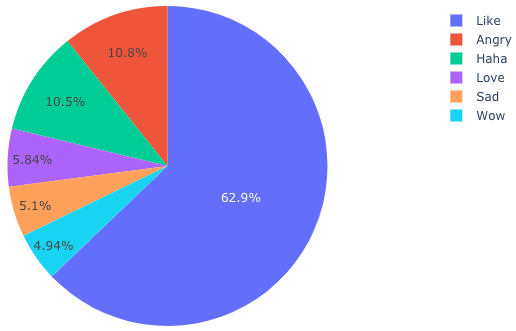
\includegraphics[width=7 cm]{reaction_percentage}
\captionof{figure}{Percentage of each type of reaction in the dataset.}\label{fig:b}
\endgroup

The number of minutes it takes for a post to get 100 comments appears to have a heavily skewed distribution with a long tail, as shown in Figure~\ref{fig:a} (a). 80.9\% of the posts get their first 100 comments within 67 hours. After applying the reciprocal root transform, the distribution appears to be normal. This is shown in Figure~\ref{fig:a} (b). The distributions of other features are also similarly skewed. 

In Figure~\ref{fig:c}, the rows indicating the fraction of "like", "angry" and "haha" reactions for each post have a higher number of brightly colored cells as compared to the rows indicating the fraction of "love", "sad" and "wow" reactions. The majority of reactions on each post are therefore "like", "angry" and "haha" reactions. This is in agreement with Figure~\ref{fig:b}, which indicates that "love", "sad" and "wow" reactions occur less frequently across the entire dataset. 
\end{multicols}
\begin{figure*}[htp]
    \begin{subfigure}{0.5\textwidth}
      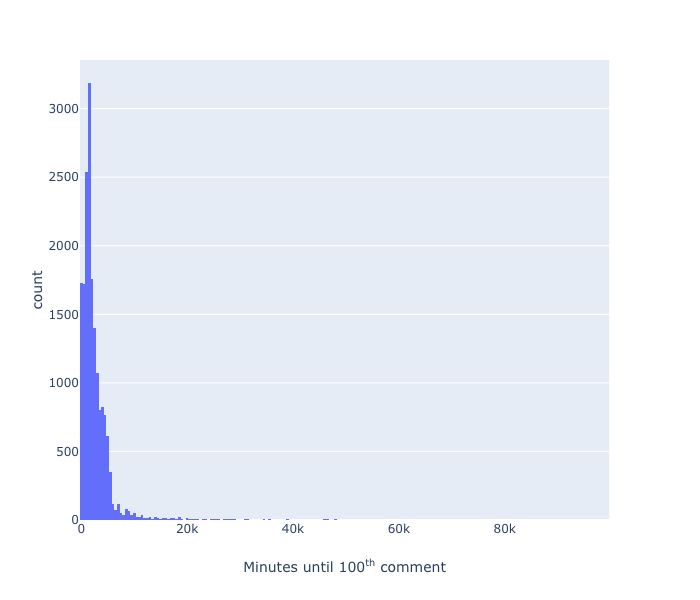
\includegraphics[width=8cm]{mins_100_skewed}
      \caption{}
    \end{subfigure}%
    \begin{subfigure}{0.5\textwidth}
      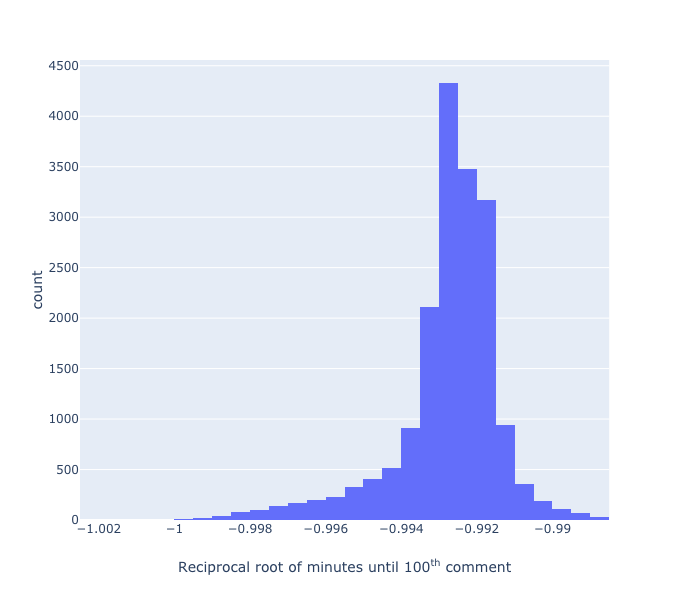
\includegraphics[width=8cm]{mins_100_transformed}
      \caption{}
    \end{subfigure}
  \caption { Distribution of the minutes it takes for a post to get 100 comments (a) before transformation (b) after transformation }\label{fig:a}
\end{figure*}
\begingroup
\centering
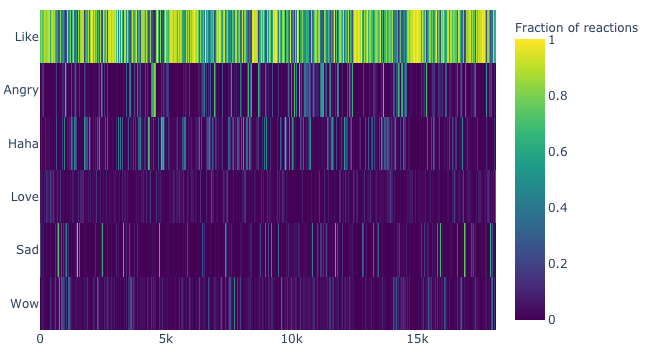
\includegraphics[scale=0.75]{reaction_fraction_all_posts}
\captionof{figure}{Fraction of each type of reaction (y-axis) for each post in the dataset (x-axis)}\label{fig:c}
\endgroup

\begin{multicols}{2}
The fraction of each type of reaction on a post indicates the sentiment of a post. As shown in Table~\ref{tab:sentiment}, posts tagged with positive sentiment (>= 0.5) by VADER  have a smaller fraction of "angry" and "sad" reactions, and a larger fraction of "love" reactions than posts tagged with negative sentiment (<=-0.5). 

\begin{center}
\captionof{table}{Relationship between sentiment of posts and the average fraction (over all posts) of reactions of each type}\label{tab:sentiment}
   \begin{tabular}{|p{1.5cm}|p{1cm}|p{1cm}|p{1cm}|}
       \hline \textbf{VADER Sentiment} & \textbf{"angry" and "sad" fraction} & \textbf{"love" fraction} & \textbf{"haha" fraction} \\
      \hline {>=0.5} & 0.107 & 0.052 & 0.079 \\
      \hline {<=-0.5} & 0.233 & 0.027 & 0.073 \\
      \hline
   \end{tabular}
\end{center}

Figure~\ref{fig:d} shows that the number of "sad" and "angry" reactions per second reduce, and the number of "love" reactions per second increase, for posts with more positive sentiment. "Wow" reactions seem to indicate negative sentiment since the rate at which they are obtained reduces as posts become more positive. Similarly, "haha" reactions seem to indicate positive sentiment. 

Figure~\ref{fig:e} shows box plots of the minutes until a post gets it's first and it's 100\textsuperscript{th} comment, for sentiment bins of width 0.1. The maximum number of minutes until both the first and 100\textsuperscript{th} comment for each bin appear to increase for bins with more positive sentiment. The median number of minutes until both the first and 100\textsuperscript{th} comment for each bin also appear to increase for bins with more positive sentiment, but not as much as the maximum. Posts therefore appear to be more popular if they are associated with more negative sentiment. Posts which get their first comment later than 6 minutes and their 100\textsuperscript{th} later than 4000 minutes (67 hours) (i.e. ~20\% of the posts) contribute more to this trend than the other 80\% of posts.
\end{multicols}
\begingroup
\centering
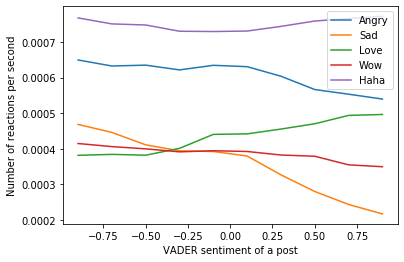
\includegraphics[scale=0.9]{sentiment_reactions}
\captionof{figure}{Variation of the number of reactions of each type obtained per second, with the VADER sentiment of a post}\label{fig:d}
\endgroup
\begingroup
\centering
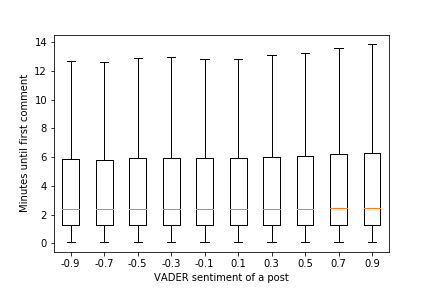
\includegraphics[scale=0.6]{images/sentiment_first_comment_box}
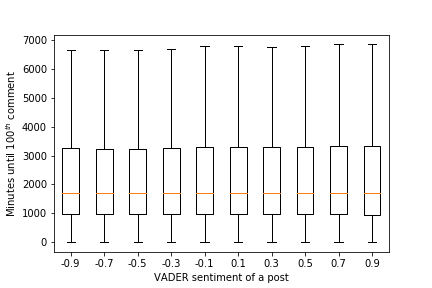
\includegraphics[scale=0.6]{sentiment_100_comment_box}
\captionof{figure}{Variation of the number of the number of minutes until the first and 100\textsuperscript{th} comment, with the VADER sentiment of a post}\label{fig:e}
\endgroup
\begin{multicols}{2}
Figures ~\ref{fig:f} (a) and ~\ref{fig:g} (a) show the variation in the R\textsuperscript{2} score and RMSE of the multivariate linear regression model (in one of the hundred iterations) as each feature is added. The R\textsuperscript{2} score sees an overall increase and the RMSE sees an overall decrease as features are added. This indicates the model performs better as more features are added. 

Some features increase the R\textsuperscript{2} score more than the others (and decrease the RMSE more than the others), as shown in Figures ~\ref{fig:f} (b) and ~\ref{fig:g} (b). It is interesting to note that the feature that leads to the largest increase in the R\textsuperscript{2} score (the number of "sad" reactions a post receives per second) is not the same as the features that decreases the RMSE the most (the number of "love" reactions a post receives per second). 

Across all 100 iterations, the six features which increase the R\textsuperscript{2} score by the largest magnitude, the maximum number of times, are the log-scaled number of "love", "sad", "like" and "wow" reactions received by a post per second, the reciprocal root transformed number of reactions per second, and minutes until a post gets its first comment.
\end{multicols}
\begin{figure*}[htp]
\centering
    \begin{subfigure}{0.9\textwidth}
      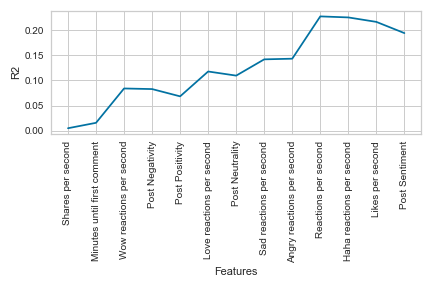
\includegraphics[scale=0.8]{r2_stepwise}
      \caption{}
    \end{subfigure}%
    \par
    \begin{subfigure}{0.9\textwidth}
      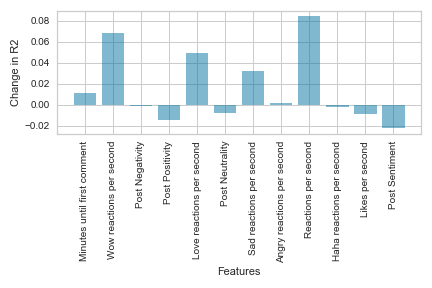
\includegraphics[scale=0.9]{r2_stepwise_change}
      \caption{}
    \end{subfigure}
  \caption { (a) Variation in the R\textsuperscript{2} score of the multivariate linear regression model as each feature is added (b) Magnitude of change in the R\textsuperscript{2} due to each feature }\label{fig:f}
\end{figure*}
\begin{figure*}[htp]
\centering
    \begin{subfigure}{0.9\textwidth}
      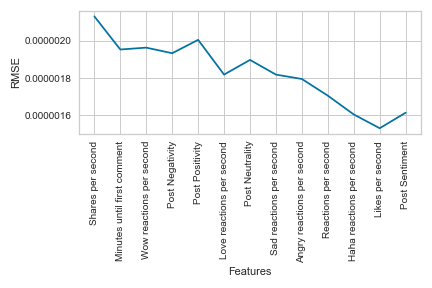
\includegraphics[scale=0.9]{mse_stepwise}
      \caption{}
    \end{subfigure}%
    \par
    \begin{subfigure}{0.9\textwidth}
      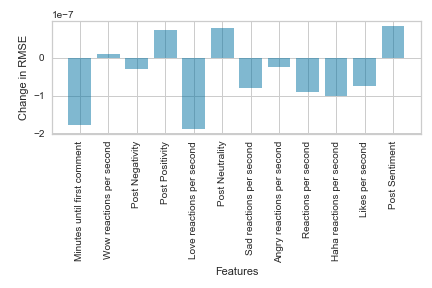
\includegraphics[scale=0.9]{mse_stepwise_change}
      \caption{}
    \end{subfigure}
  \caption { (a) Variation in the RMSE of the multivariate linear regression model as each feature is added (b) Magnitude of change in the RMSE due to each feature }\label{fig:g}
\end{figure*}
\clearpage
\begin{multicols}{2}
Table~\ref{tab:coeffs} shows the coefficients and the p-values for multivariate linear regression for one iteration. The features with p-values $\gg \alpha$ $(\alpha = 0.05)$ are post negativity, positivity, neutrality and sentiment. These are the same features that lead to a decrease in the R\textsuperscript{2} score and an increase in the RMSE (Figures ~\ref{fig:f} and ~\ref{fig:g}). 

Figure ~\ref{fig:coeffs} shows the log-scaled absolute values of the same coefficients. Features with significant coefficients don't always lead to an increase in the R\textsuperscript{2} score (for example, the post positivity) and features with less significant and negative coefficients do lead to an increase in the R\textsuperscript{2} score (for example, minutes until the first comment and the number of "wow" reactions per second). 

For SVR, a grid search was performed over three kernels (linear, RBF and polynomial), four values of $C$ (0.1, 1, 100, 1000), eleven values of $\epsilon$ (0.0001, 0.0005, 0.001, 0.005, 0.01, 0.05, 0.1, 0.5, 1, 5, 10) and seven values of $\gamma$ (0.0001, 0.001, 0.005, 0.1, 1, 3, 5). The RBF kernel with values $C=0.1$, $\gamma=0.1$ and $\epsilon=0.0001$ performed the best. 

A comparison of the performance of the three chosen models (Table~\ref{tab:b}) indicates that MARS improves the R\textsuperscript{2} score by 12.7\% over Multivariate Linear Regression, and SVR further improves it by 14.2\%. MARS reduces the RMSE by 5.4\%.
\end{multicols}

\begin{table}
\centering
   \caption{Multivariate linear regression coefficients and p-values for one iteration} \label{tab:coeffs}
   \begin{tabular}
      {lll} \hline \textbf{Feature} & \textbf{Coefficient (in reciprocal root transformed minutes)} & \textbf{P-value} \\
      \hline {Likes per second} & {-0.0010} & {$\ll 0.001$}\\
      \hline {Post negativity} & {-0.0176} & {0.701}\\
      \hline {Reactions per second} & {0.2091} & {$\ll 0.001$}\\
      \hline {Shares per second} & {0.0157} & {$\ll 0.001$}\\
      \hline {Minutes until first comment} & {-0.0009} & {$\ll 0.001$}\\
      \hline {"Wow" reactions per second} & {-0.0004} & {$\ll 0.001$}\\
      \hline {"Angry" reactions per second} & {-0.0002} & {$\ll 0.001$}\\
      \hline {"Love" reactions per second} & {-0.0008} & {$\ll 0.001$}\\
      \hline {"Haha" reactions per second} & {-0.0003} & {$\ll 0.001$}\\
      \hline {Post positivity} & {-0.0180} & {0.695}\\
      \hline {"Sad" reactions per second} & {-0.0005} & {$\ll 0.001$}\\
      \hline {Post neutrality} & {-0.0177} & {0.700}\\
      \hline {Post sentiment} & {$4.58 \times 10^{-5}$} & {0.297}\\
      \hline
   \end{tabular}
\end{table}
\begin{table}
   [ht] \caption{Performance of regression models} \label{tab:b}
   \begin{tabular*}{\textwidth}{c @{\extracolsep{\fill}} ccc}
      \hline \textbf{Model} & \textbf{R\textsuperscript{2} Score} & \textbf{RMSE} \\
      \hline Multivariate Linear Regression & 0.212 & $1.65 \times 10^{-6}$ \\
      \hline MARS & 0.239 & $1.56 \times 10^{-6}$  \\
      \hline SVR & 0.273 & $1.58 \times 10^{-6}$  \\
      \hline
   \end{tabular*}
\end{table}
\clearpage
\begingroup
\centering
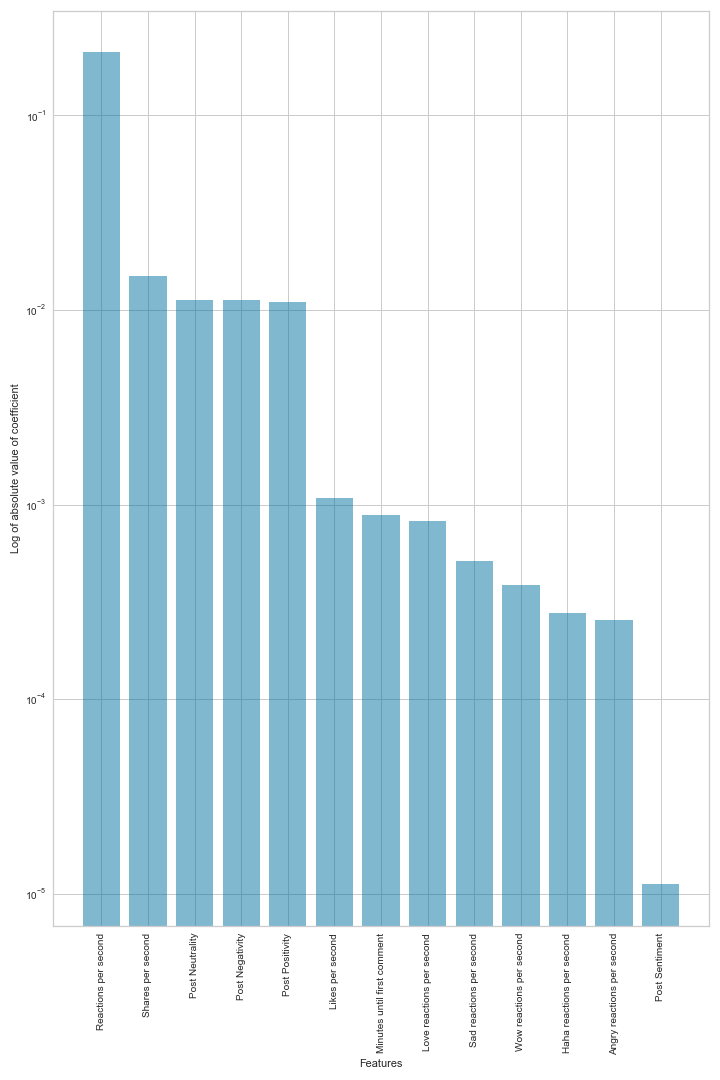
\includegraphics[scale=0.5]{images/multi_lr6_abs_coeffs_log}
\captionof{figure}{Log-scaled absolute values of coefficients for multivariate linear regression (one iteration)}\label{fig:coeffs}
\endgroup
\begin{figure*}[htp]
\centering
    \begin{subfigure}{0.7\textwidth}
      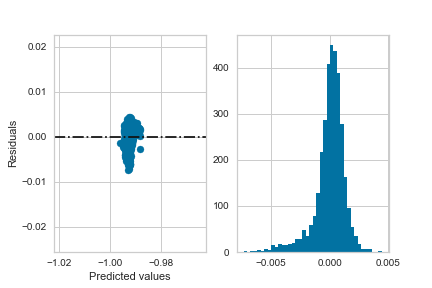
\includegraphics[scale=0.65]{multireg_residuals}
      \caption{}
    \end{subfigure}%
    \par
    \begin{subfigure}{0.7\textwidth}
      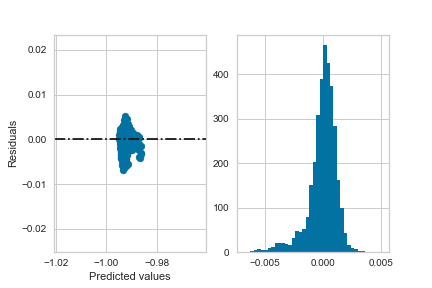
\includegraphics[scale=0.65]{mars_residuals}
      \caption{}
    \end{subfigure}
    \par
    \begin{subfigure}{0.7\textwidth}
      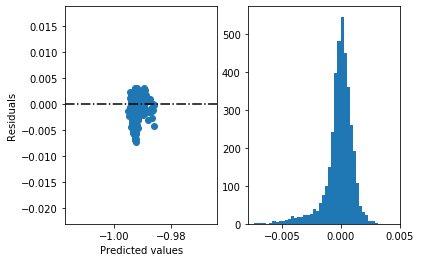
\includegraphics[scale=0.65]{svr_residuals}
      \caption{}
    \end{subfigure}%
  \caption { Residuals and their distribution for each of the three models (a) Multivariate linear regression (b) MARS (c) SVR }\label{fig:residuals}
\end{figure*}
\clearpage
\begin{multicols}{2}
Figure ~\ref{fig:residuals} shows that the distributions of residuals become progressively narrower and more heavy tailed. This could indicate that multivariate linear regression gives the outliers just as much importance as the other observations, thus leading to more data points having larger residuals (a wider distribution) and the outliers having smaller residuals (a distribution with no long tails). MARS and SVR, on the other hand, give the outliers less importance. The non-outliers therefore fit better (smaller residuals, narrower distribution) but the outliers have large residuals, which leads to the heavy tails in the distribution.
\end{multicols}
\begingroup
\centering
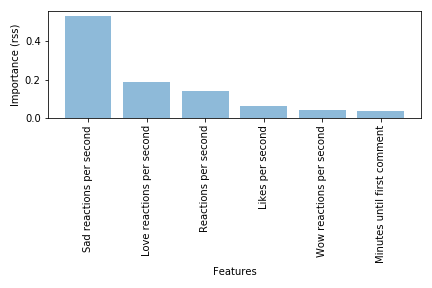
\includegraphics[scale=0.7]{images/mars_imp_rss}
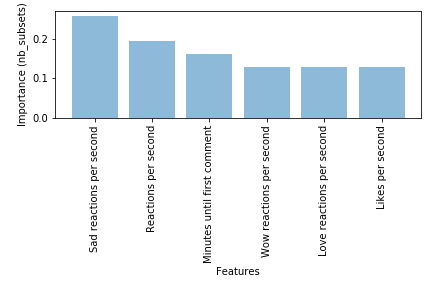
\includegraphics[scale=0.7]{mars_imp_nb_subsets}
\captionof{figure}{Features that MARS chose to be the most predictive with RSS and number of model subsets as measures of importance respectively}\label{fig:marsimportances}
\endgroup
\begin{multicols}{2}
For the MARS model, feature importance can be measured either by the residual sum of squares (RSS) or the number of model subsets that include the feature [7]. Figure ~\ref{fig:marsimportances} shows that the number of "sad" reactions received by a post per second is chosen to be the most predictive feature, using both RSS and number of subsets as the criteria. 

On the other hand, the multivariate linear regression model chose the number of (all types of) reactions to be the most predictive, thereby disregarding the sentiment of the post in determining its popularity (Figure ~\ref{fig:coeffs}). The total number of reactions a post receives per second could be a measure of the number of followers a news page has and the number of friends each of those followers has. The greater these two are, the greater the number of feeds on which the post shows up, which leads to more people reacting to the post. The multivariate linear regression model therefore seems to use the popularity of a news page and its followers to determine the popularity of a post. 

The MARS model assigns small weights to reactions per second, likes per second and minutes until the first comment, all of which do not take the sentiment of a post into account.  The number of "sad" reactions per second takes both of the page popularity and post sentiment into account. The MARS model therefore appears to determine the popularity of a post not only by the popularity of the news page the post is on and the popularity of its followers, but also by the sentiment of the post. 

It is also interesting that the MARS model considers the number of "sad" reactions to be more predictive than the number of "love" reactions per second to predict popularity. This could mean people react to posts with negative sentiment but don't react to posts with positive sentiment. Positive sentiment is then indicated by the absence of negative reactions, rather than by the presence of positive ones. It is also interesting to note that the multivariate linear regression coefficients with largest magnitude include the number of reactions per second, the positivity, negativity and the neutrality of a post, i.e. its sentiment (Figure ~\ref{fig:coeffs}). By choosing the number of "sad" reactions per second to be the most predictive, MARS, in some sense, chooses a feature that is a combination of the most predictive features of the linear regression model.
\section{Discussion and Conclusions}
This study assessed the effects of various features such as the number and type of reactions received by a post per second, the sentiment of the post, etc. on the popularity of the post. The sentiment of a post was found to influence the popularity of a post more than the popularity of the page the post was created on or the popularity of its followers. In line with previous research, posts with negative sentiment were found to be more popular. 

The feature importances assigned by the RBF SVR kernel could not be calculated as it transforms the features to a more complex space and then assigns weights. A possible extension to this study would be to determine what features the RBF kernel chose to be the most predictive. In addition to this, the six features that lead to the most increase in the R\textsuperscript{2} score of the multivariate linear regression model were used to train the MARS and SVR models. Choosing the features with the highest values of multivariate linear regression coefficients could lead to different results and provide different insights into the popularity of posts. 
%----------------------------------------------------------------------------------------
% REFERENCE LIST
%----------------------------------------------------------------------------------------
\begin{thebibliography}{9}
\bibitem{banerjee2019} 
Banerjee, S. and Chua, A.Y.K. J Brand Manag (2019) 26: 621. \textit{https://doi-org.colorado.idm.oclc.org/10.1057/s41262-019-00157-7}.
\bibitem{bo2015}
Bo Wu, Haiying Shen, (2015). Analyzing and predicting news popularity on Twitter,
International Journal of Information Management.
\textit{https://doi.org/10.1016/j.ijinfomgt.2015.07.003.}.
\bibitem{ferrara2015}
Ferrara E, Yang Z. 2015. Quantifying the effect of sentiment on information diffusion in social media. PeerJ Computer Science 1:e26 
\textit{https://doi.org/10.7717/peerj-cs.26}.
\bibitem{gelli2015}
Francesco Gelli, Tiberio Uricchio, Marco Bertini, Alberto Del Bimbo, and Shih-Fu Chang. 2015. Image Popularity Prediction in Social Media Using Sentiment and Context Features. In Proceedings of the 23rd ACM international conference on Multimedia (MM '15). ACM, New York, NY, USA, 907-910. 
\textit{DOI: https://doi.org/10.1145/2733373.2806361}
\bibitem{fbnews2017} 
John Bencina, 2017.
\textit{Facebook News Scraper https://github.com/jbencina/facebook-news}. 
\bibitem{trans2001} 
James Kirchner, 2001.
\textit{Data Analysis Toolkit \#3: Tools for Transforming Data http://seismo.berkeley.edu/\~kirchner/eps\_120
/Toolkits/Toolkit\_03.pdf}.
\bibitem{trans2001} 
Stephen Milborrow, 2019.
\textit{Notes on the earth package  
http://www.milbo.org/doc/earth-notes.pdf}.
\end{thebibliography}
%----------------------------------------------------------------------------------------
\end{multicols}
\end{document}